\documentclass[a4paper,10pt]{article}
\usepackage[utf8]{inputenc}
\usepackage[T1]{fontenc}
\usepackage[ngerman]{babel}
\usepackage{markdown}
\usepackage{graphicx}
\usepackage{tikz-uml}
\usepackage{float}
\usepackage{hyperref}
\usepackage[section]{placeins}

%opening
\title{Anforderungsanalyse}
\author{Julian Hildebrand\and{}Julian Wasilewski\and{}Lukas Pöhler\and{}Christoph Raitzig}
    
\begin{document}

\maketitle

\tableofcontents

\newpage

\section{Mock-Ups}
Die Weboberfläche braucht 3 Seiten.\\
In Abb. \ref{dashboard} ist das Mock-Up fürs Dashboard zu sehen. In Abb. \ref{jobs} ist das Erstellen bzw. Bearbeiten von Jobs dargestellt. In Abb. \ref{logs} kann man Logs sehen.
\begin{figure}[!htb]
	\centering
	\includegraphics[width=\textwidth]{../Mock-Ups/mockup-dashboard}
	\caption{Dashboard}
	\label{dashboard}
\end{figure}
\begin{figure}[!htb]
	\centering
	\includegraphics[width=\textwidth]{../Mock-Ups/mockup-jobs}
	\caption{Jobs erstellen bzw. bearbeiten}
	\label{jobs}
\end{figure}
\begin{figure}[!htb]
	\centering
	\includegraphics[width=\textwidth]{../Mock-Ups/mockup-logs}
	\caption{Logs/Historie}
	\label{logs}
\end{figure}

%\section{Use-Cases}
\input{usecases.tex}

\section{Komponentendiagramm}
Das Komponentendiagramm ist in Abb. \ref{komponentendiagramm} dargestellt. Der direkte Zugriff auf die Datenbankschnittstelle ohne das Backend als prüfende Instanz beinhaltet ein gewisses Risiko. Nach Rücksprache mit dem Auftraggeber wurde abgeklärt, dass bereits vorher eine Authentifizierung der Nutzer stattfindet und den angemeldeten Nutzern vertraut werden kann.
\begin{figure}[!htb]
	\centering
	\includegraphics[width=\textwidth]{../Components}
	\caption{Komponentendiagramm}
	\label{komponentendiagramm}
\end{figure}

\section{Datenbank-ER-Diagramm}
Das ER-Diagramm der Datenbank ist in Abb. \ref{dber} dargestellt.
\begin{figure}[!htb]
	\centering
	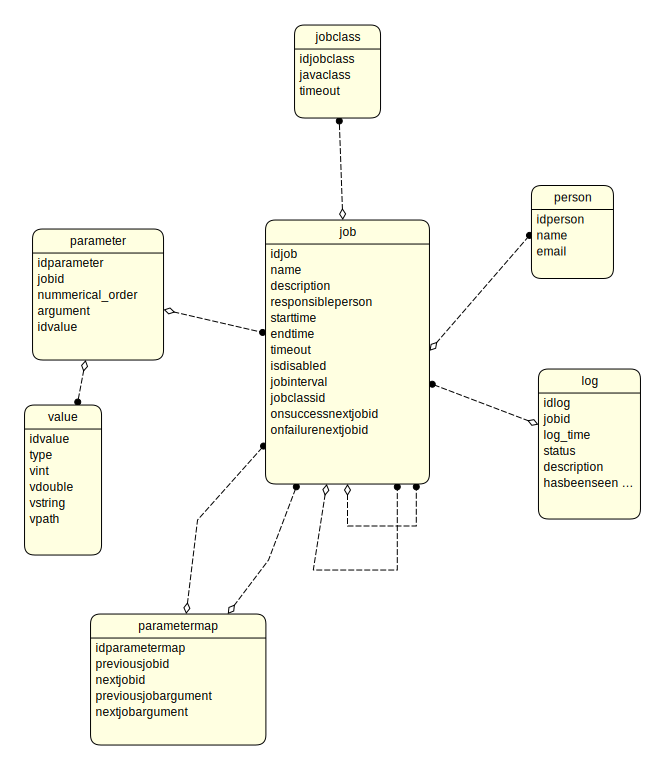
\includegraphics[width=\textwidth]{ER-Diagramm}
	\caption{ER-Diagramm}
	\label{dber}
\end{figure}

\section{Klassendiagramm}
\subsection{Backend}
\resizebox{\textwidth}{!}{
	\begin{tikzpicture}
	\begin{umlpackage}[x=0, y=0]{jobs}
	\umlclass[x=0, y=0,type=interface]{JobInterface}{}{
		+run() : JobResult\\ +setId(id : int)\\ +getId() : int\\ +setName(name : String)\\ +getName() : String\\ +setDescription(description : String)\\ +getDescription() : String\\ +setResponsiblePerson(person : Person)\\ +getResponsiblePerson() : Person\\ +setStartTime(start : Date)\\ +startTime() : Date\\+setEndTime(end : Date)\\ +endTime() : Date\\ +getStatus() : int[]\\ +hasTimeout() : boolean\\ +getTimeout() : long\\ +setTimeout(timeout : long)\\ +setParameters(params : JobParameter[]) : boolean\\ +setParametersFromJob(params : JobParameter[]) : boolean\\ +getParameters() : JobParameterInfo[]\\ +setNextOnSuccess(nextJob : JobInterface)\\ +setNextOnFailure(nextJob : JobInterface)\\ +setInterval(interval : String)\\ +interval() : String\\ +stop()\\ +isStopped() : boolean\\ +abort()\\ +nextOnSuccess() : JobInterface\\ +nextOnFailure() : JobInterface\\ +nexParams() : JobParameter[]
	}
	\umlclass[x=14,y=1.4]{Person}{
		-name : String\\ -email : String
	}{
		+Person(name : String, email : String)\\ +getName() : String\\ +getEMail() : String
	}
	\umlclass[x=0,y=-11]{JobResult}{
		-success : boolean\\ -message : String\\ -result : Byte[]\\ -MIMEType : String\\ -outputParams : JobParameter[]
	}{
		+JobResult()\\ +JobResult(success: boolean, message : String)\\ +hasSucceded() : boolean\\ +getMessage() : String\\ +getResult() : Byte[]\\ +getMIMEType() : String\\ +getParams()
	}
	\umlclass[x=10,y=-4]{JobParameter}{
		-type : ParameterType\\ -name : String\\ -intP : int\\ -doubleP : double\\ -stringP : string\\ -fileId : int
	}{
		+JobParameter(name : String, i : int)\\ +JobParameter(name : String, d : double)\\ +JobParameter(name : String, s : String)\\ +JobParameter(name : String, fileId : int, nothing : boolean)\\ +getType() : ParameterType\\ +getName() : String\\ +getInt() : int\\ +getDouble() : double\\ +getString() : String\\ +getFileId() : int
	}
	\umlclass[x=14,y=-10,type=enum]{ParameterType}{
		INT, DOUBLE, STRING, FILEID
	}{
		
	}
	\umlclass[x=8,y=-12]{JobParameterInfo}{
		-type : ParameterType\\ -name : String\\ -description : String
	}{
		+getType() : ParameterType\\ +getName() : String\\ +getDescription() : String\\ +check(i : int) : boolean\\ +check(d : double) : boolean\\ +checkId(fileId : int) : boolean\\ +check(s : String) : boolean\\ +getHint(i : int) : String\\ +getHint(d : double) : String\\ +getHintId(fileId : int) : boolean\\ +getHint(s : String) : boolean
	}
	\umlclass[x=10, y=5]{JobController}{
		\umlstatic{-jobController : JobController}\\ -jobs : ArrayList\textless{}JobInterface\textgreater{}
	}{
		-JobController()\\ \umlstatic{+getInstance() : JobController}\\ addJob(job : JobInterface) : boolean\\ +scheduleJob(job : JobInterface)\\ +scheduleJobOnce(job : JobInterface, delay : long)
	}
	\umlclass[x=8, y=1.5]{JobRunner}{
		-job : JobInterface\\ -timer : Timer
	}{
		+run()
	}
	\umlclass[x=-3, y=-17]{PingJob}{

	}{
		
	}
	\umlclass[x=0, y=-17]{RESTJob}{

	}{
		
	}
	\umlclass[x=3, y=-17]{EMailJob}{

	}{
		
	}
	\umlclass[x=6, y=-17]{CommandJob}{

	}{
		
	}
	\umlclass[x=9, y=-17]{DockerJob}{

	}{
		
	}
	\end{umlpackage}
	\begin{umlpackage}[x=-4, y=-22]{server}
	\umlclass[x=0, y=0]{Receiver}{

	}{
		+createNewJob(job : JobInterface)\\ +startJob(job : JobInterface)\\ +getDashboardInfo()\\ +getJobStatus(job : JobInterface)\\ +updateJob(job : JobInterface)
	}
	\umlclass[x=10, y=0]{DBHandler}{
		\umlstatic{-handler : DBHandler}\\ \umlstatic{-smartData : Connection}
	}{
		-DBHandler()\\ \umlstatic{+getInstance() : DBHandler}\\ +save(result : JobResult) : boolean\\ +addJob(job : JobInterface) : boolean\\ +updateJob(job : JobInterface) : boolean\\ +getLogs() : Log[]\\ +getJobs() : JobInterface[]\\ +getJob(id : int) : JobInterface\\ +existsUnseenFailure() : boolean\\ +getUnseenFailures() : JobResult[]\\ +setLogSeen(log : Log) : boolean\\ +getParameterMap() : Map<String>\\+removeParameterMap(jobPreviousId : int, jobNextId : int, map : Map<String>)\\ +addParameterMap(jobPreviousId : int, jobNextId : int, map : Map<String>)
	}
	\umlclass[x=5, y=-6.5]{Log}{
		-timestamp : Date\\ -jobName : String\\ -jobId : int\\ -success : boolean\\ -message : String
	}{
		+Log(timestamp : Date, job : JobInterface, success : boolean, message : String)\\ +getTimestamp() : Date\\ +getJobName() : String\\ +getJobId() : int\\ +getStatus() : boolean\\ +getMessage() : String
	}
	\end{umlpackage}
	\umlcompo{JobRunner}{JobInterface}
	\umlcompo{JobParameterInfo}{ParameterType}
	\umlcompo{JobParameter}{ParameterType}
	\umlaggreg{JobController}{JobInterface}
	\umlaggreg{JobResult}{JobParameter}
	\umlimpl{PingJob}{JobInterface}
	\umlimpl{RESTJob}{JobInterface}
	\umlimpl{EMailJob}{JobInterface}
	\umlimpl{CommandJob}{JobInterface}
	\umlimpl{DockerJob}{JobInterface}
	\end{tikzpicture}
}
\subsection{Frontend}
\begin{figure}[!htb]
	\centering
	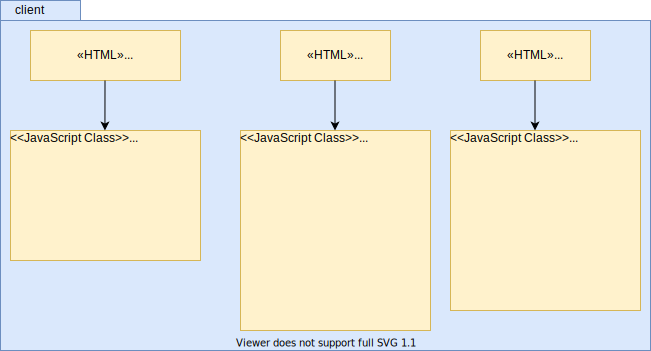
\includegraphics[width=\textwidth]{KlassendiagrammFrontend.png}
	\caption{Klassendiagramm vom Frontend}
	\label{klassendiagrammFrontend}
\end{figure}

\section{Sequenzdiagramm}
Das Sequenzdiagramm für das manuelle Starten eines Jobs ist in Abb. \ref{seqStartJobManually} dargestellt.
\begin{figure}[!htb]
	\centering
	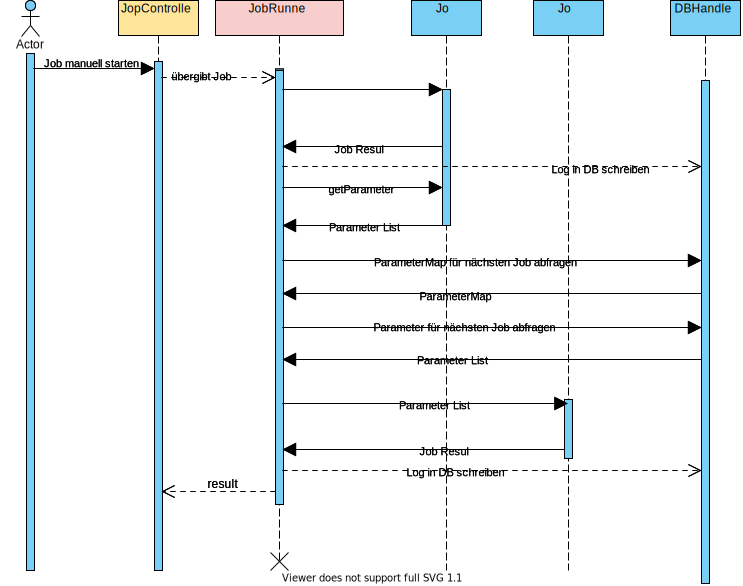
\includegraphics[width=\textwidth]{Sequenzdiagramm.png}
	\caption{Sequenzdiagramm: Job manuell starten}
	\label{seqStartJobManually}
\end{figure}

\section{Meilensteinplan}
\begin{itemize}
 \item 1. Meilenstein (1.12.2020):
 \begin{itemize}
  \item Grundgerüst der Website funktionsfähig
  \item Datenbank eingerichtet
  \item SmartData integriert
  \item Backend: Schnittstelle zum Frontend mit Dummy-Daten funktionsfähig
  \item Ergebnisse der Anfragen ans Backend werden dargestellt
  \item Kommunikation unter den Mikroservices eingerichtet
 \end{itemize}
 \item 2. Meilenstein (15.12.2020):
 \begin{itemize}
  \item Job Controller, Job Runner implementiert
  \item Job Controller kann Jobs schedulen
  \item Job Runner läuft multithreaded
  \item DB Schnittstelle implementiert
  \item Ping Job, Docker Job implementiert
  \item Schnittstelle zum Frontend mit echten Daten funktionsfähig
  \item dynamische Generierung des Dashboards mit Daten aus der DB
  \item dynamische Generierung der Job Konfiguration
 \end{itemize}
 \item 3. Meilenstein (5.1.2021):
 \begin{itemize}
  \item E-Mail Job, REST Job und Command Job implementiert
  \item Logs werden angezeigt und können gefiltert werden
 \end{itemize}
\end{itemize}

\section{Aufgabenverteilung}
Frontend:
\begin{itemize}
 \item Julian Hildebrand
 \item Lukas Pöhler
\end{itemize}
Backend:
\begin{itemize}
 \item Julian Wasilewski
 \item Christoph Raitzig
\end{itemize}
Sonstiges:
\begin{itemize}
 \item Docker-Container einrichten: Julian Hildebrand
\end{itemize}

\end{document}
